\chapter{Background Study}
\label{chap:2}

This chapter contains background information on the software, services and algorithms used
in this project. They are divided up into Quick Response Codes (QR Codes), Near Field
Communication (NFC), the web server and the encryption algorithms used.

\section{Quick Response Codes}

 Quick Response Codes (QR Codes) are two dimensional bar codes that were initially
 used in Japanese car factories to allow computers to track the progress of
 an item on a production line [\cite{journal:qr-code}]. The technology has
 since evolved and matured and is today widely used in the media industry for storing
 data, such as a web address or a phone number. See Figure \ref{qrcode} for an example of
 a QR code.
 
\begin{figure}
\centering
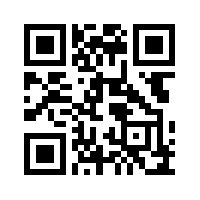
\includegraphics[scale = 0.7]{qrcode_voorbeeld.png}
\caption{Example of a QR Code.}
\label{qrcode}
\end{figure}
 
 QR Codes can store up to 7089 alphanumeric characters [\cite{journal:qr-code}], which are
 accessible by scanning the code with either a laser or a digital camera.
 Scanning a QR Code requires a camera that can produce a digital image at a
 resolution that is at least twice that of the QR Code.
 This image is then processed by a QR Code library, e.g.
 the ZXing library (see section \ref{sec:zbar} for more detail on the ZXing library),
 which decodes the picture and extracts the data embedded inside the code. Cellphones are
 commonly used today because of their portability, increasingly powerful hardware and QR
 Code technology's simplicity.
 However, an image with an embedded QR Code can be decoded by any computer with the
 necessary hardware and libraries installed, e.g. a webcam and the ZXing
 library.

\subsection{Zebra Crossing Library}
\label{sec:zbar}

The Zebra Crossing Library (ZXing for short) is a QR Code coding and decoding
library [\cite{website:zxing}]. It is commonly built into smart phone
applications to decode QR Codes embedded inside a static image or a video
stream. A desktop version of the library, called ZBar, is also available and
works in a similar manner.

The Barcode Scanner application is made by the team that made the ZXing
library. It is freely available on multiple cellphone platforms, such as
BlackBerry OS, Apples's iOS and Google's Android. 

To date there have been at least 50 million downloads of
ZXing's Barcode Scanner application on the Android platform alone, and it
currently lies 98$^{\rm th}$ in the top 100 of the Google Play Store's most
downloaded list [\cite{website:barcodescanner}]. This shows the extent to which
QR Code technology and the ZXing library has evolved to be used by millions of
people.

\section{Near Field Communication}

Near Field Communication (NFC) is a relatively new communication standard in the world of
wireless technology. It allows two NFC-enabled devices to wirelessly transmit data by bringing
them close to one another, typically around 4 centimeters.

Most mainstream cellphone manufacturers, with the major exception of Apple, have
added NFC capabilities to their flagship models, and more recently to some of
their budget models [\cite{website:nfc-models}]. 

The technology has also been
ported to other platforms, such as the desktop computer and Arduino. This adds a
new dimension to wireless inter-device communication and makes projects such as
this more feasible.

\subsection{libnfc}

Libnfc is an open-source library for Linux systems [\cite{website:libnfc}]. It allows a
desktop computer to communicate with a NFC device which is based on the Phillips PN53
series of NFC chips [\cite{website:libnfc-hardware}]. Recent versions have made provision
for the use of a PN532 breakout board that can be used by a Raspberry Pi. 

It is currently in version 1.7 and is classified as a `mature' library by the
open-source community.

\subsubsection{nfcpy}
\label{sec:nfcpy}

Nfcpy is a Python interface for the libnfc library and it allows for peer-to-peer communication
between a cellphone and desktop-based NFC controller using the NFC Data Exchange Format
(NDEF), the Simple NDEF Exchange Protocol (SNEP) and the Logical Link Control Protocol (LLCP).
These standards and protocols have been set by the NFC standard governing body, the NFC Forum
[\cite{website:nfc-forum}], to simplify and standardise data exchange between different
platforms and to make the user experience more pleasant.

Nfcpy is an open-source program, written and maintained by Stephen Tiedemann
[\cite{website:nfcpy}].

\subsection{Android}

Google's Android operating system is currently the most widely used cellphone operating
system world wide, with an estimated 80\% market share
[\cite{article:android-marketshare}].
Other platforms, such as the Blackberry OS and Windows Phone, have also added NFC to their
latest phones, but they do not have the market penetration that Android currently has and it
was found that application development on the Android platform is relatively simple and free.

Android is also the platform which most actively promotes the use of NFC as an
alternative payment option in modern retail outlets, with applications such as Google Wallet
[\cite{article:android-wallet}] being heavily promoted by Google.

\subsection{Radio Field Identification and Stellenbosch
University Student Cards}

NFC and Radio Frequency Identification (RFID) work in a similar manner: when two
devices  (e.g. cellphone, RFID tag, MiFare card, etc.), equipped with an antenna
tuned to a certain frequency, for example 13.56 MHz, come into close
proximity, they transmit some form of data to one another.

However, there are some important difference between the two technologies. For example, a NFC
system is  an active system, meaning that the device's antenna is always powered and runs off
its own  power supply. NFC devices also have peer-to-peer (p2p) capabilities, meaning that the
two  devices can communicate with one another by both sending and receiving data.
RFID systems on the  other hand, work by having one device act as a listener and the other as a
sender [\cite{article:diff-nfc-rfid}] (e.g. the current SU's student entry control system).

\section{Web Server}

The web server is responsible for handling all the data transfers and transactions that
take place when a customer buys a product. 

In this section, some background information will be given on
the key features of the web server that was implemented for this project.

\subsection{Django Web Framework}
\label{sec:django}

Django is a Python web server framework which focuses on easy setup and simple design. Here are
some of its features:

\begin{itemize}
  \item Fully handles Hypertext Transfer Protocol (HTTP) GET and POST requests.
  \item Integrates with SQL databases, e.g. MySQL, SQLite3, etc.
  \item Supports Hypertext Markup Language (HTML) template design.
  \item Makes provision for the execution of Python scripts.
  \item Is fully scalable to commercial level servers.
  \item Has an offline server debugging function available.
\end{itemize}

This framework is expandable to commercial size servers that are accessible across the
globe. For example large websites such as Instagram and Pinterest are based on the Django
framework [\cite{website:django-sites}].

To make it easier to program, read and debug, the original Django developers
designed Django to split its websites into multiple so-called `applications'.
These applications typically contain a single web-page with its own script and
database handling functionality. These applications can communicate with one
another, meaning that one script from application X may execute a script or
call a function in application Y.

Django was initially developed by web programmers Adrian Holovaty and Simon Willison, from the
newspaper Lawrence Journal World [\cite{website:django-exist}]. It was first released in 2005
under the Berkeley Software Distribution (BSD) license and is completely free to use.

\subsection{Elastic Compute Cloud}
\label{sec:ec2}

Elastic Cloud Compute (EC2) is a cloud computing service offered by Amazon Web
Services (AWS) [\cite{website:aws}]. It allows a user to rent a cloud-based
virtual computer from AWS from which to run their own applications.
These applications are commonly web-based, in other words the virtual machines run a
web server that is accessible by anyone around the world.  

AWS offers new users the option to create a virtual machine for free. These free
virtual machine instances are limited to the least powerful machine tier available, but
functionally the free and paid tiers work the same.

\subsection{Apache}
\label{sec:apache}

Apache is a popular web server application available on most operating system
platforms [\cite{website:apache-platforms}].
A very notable feature of Apache is that it was designed to be easily
configurable. This makes it easier to run various web frameworks off of it, such
as Python's Django, PHP's cgiapp and C++'s Poco.

Apache is the most widely-used web server framework in use today, with an
estimated 53.4\% of the world's servers running on it [\cite{website:apache-usage}].

It was initially released by Robert McCool in 1995 under the Apache Licence, which makes it
free to use in any way. It is currently being maintained by the Apache Software
Foundation [\cite{website:apache}].

\section{Encryption}

Encryption is the act of encoding some data into a form that is intended to be
unintelligible to anyone other than the intended recipient.
This is done to ensure that only authorised parties can access sensitive data.
This is most commonly done with an encryption key and an algorithm which
specifies how the data was encoded and how it can be decoded.

Encryption is commonly used where sensitive information is being transmitted between
two remote parties, e.g. banking codes, personal e-mails, etc.

Two main encryption schemes were considered for this project. They are symmetric
and asymmetric encryption and they are discussed in this section.

\subsection{Symmetric Encryption}

In symmetric encryption, both parties, i.e. the sender and receiver, have to agree to a common
encryption key prior to the data transmission. In other words, the sender and receiver use the
same key to encrypt and decrypt the data [\cite{article:symm-encryption}]. A famous example
of symmetric encryption is the Enigma cipher machine used by Nazi Germany
during the Second World War [\cite{article:enigma}].

Unfortunately, due to the increase in knowledge and understanding around this type of
encryption and the increase in modern computing power, various code cracking
methods, such as known and chosen plain-text attacks 
[\cite{journal:cypher-attacks}]. have been developed since 1945 that can break
the most commonly used symmetric encryption methods. Methods, such as the
One-Time Pad (OTP) encryption, are still being used today and is considered to
be unbreakable [\cite{article:otp}]. However, the difficulty of securely
exchanging the keys between the communicating parties is difficult
[\cite{article:otp}].

\subsection{Asymmetric Encryption}
\label{sec:assymetric-encryption}

Another encryption scheme is asymmetric encryption, or public-key
encryption. It involves the use of a public and private key pair that can be
used to securely encrypt and sign a data package on the sender's side and to
decrypt and verify the data and its origin on the receiver's side
[\cite{article:pub-encryption}].

These private and public keys are mathematically related to one another
according to the algorithm in use (e.g. ElGamal or RSA. See sections
\ref{sec:elgamal} and \ref{sec:rsa} for more information on these algorithms).
The public key is used to encrypt data and may be publicly distributed. However,
in practise the keys are only distributed to trusted parties to increase security.
The great advantage of asymmetric encryption is that even if the public half of the key is
available, it is still very difficult, and sometimes impossible, to get the
private half of the key from the public key alone.

The private key allows one to decrypt the data encrypted with the public half of the key.

The encryption is most easily explained with a postal analogy:

Imagine that two people, Alice and Bob, want to send each other secret messages through
the public mail. In other words, Alice wants to send Bob a secret message and she expects
a secret reply from Bob, and vice versa. 

In an asymmetric scheme, Bob can lock his letter to Alice with a padlock to which only she has
a key (she keeps this on her person at all times and does not show it to anyone, which
includes Bob). This open padlock represents the public key half of Alice's key. This
means that anyone can send Alice a secure message with a public key, which is easy to
get from Alice, and only Alice can unlock the message with her private key half of the
key pair. Similarly, Alice can lock her letter with Bob's padlock which only Bob can open.

The great advantage that this has over symmetric encryption is that the decryption keys never
have to be exchanged between parties. This neutralises the risk of a middle-man attack,
analogous to a nosy postal worker called Eve who likes to read other people's
mail, who then intercepts the message and steals the key. Also, if for example Bob has
been careless and allowed Eve to see his key, his messages to Alice will be
compromised. However, the messages from anyone else (including Bob) to Alice
will remain as secure as it was before Bob lost his key.

The data source can also be signed and verified by using this key scheme. Referring once again
to the postal analogy:

To show Alice that it was indeed Bob who sent her the message, and not Eve for example, he can
send an extra message along with the original message. This extra message is locked with Bob's
key that he shares with no one (i.e. his private key). However, Bob has sent out his
public key to everyone who wants it. These keys can \emph{only} be used to unlock
the messages locked with Bob's own private key. Therefore, if Alice, who received one of Bob's keys, can unlock this extra
message with that key, she knows that as long as Bob has not given anyone his
private key, it can only be his message. The reverse is also true if Alice
wants to prove to Bob that it was indeed she who sent him a message. 

\subsubsection{ElGamal}
\label{sec:elgamal}

The ElGamal encryption algorithm is an alternative to the more widely used  Ron Rivest, Adi
Shamir and Leonard Adleman (RSA) asymmetric encryption algorithm. ElGamal's security stems
from the `difficulty of computing discrete logarithms in a large prime modulus'.
[\cite{website:elgamal}]

The main advantage that the ElGamal algorithm has over RSA is that, firstly, a smaller key can
be used for a data string of the same length and secondly, due to the mathematics behind the
algorithm, it is almost certain that a different ciphertext will be generated each time a
string is encrypted.

However, a fairly large drawback of this algorithm is that the key needs to be at least twice
as long as the plain-text string that is being encrypted
[\cite{journal:elgamal}].

The algorithm was developed by Taher ElGamal in 1984 and is free to use under the GNU license.

\subsubsection{RSA}
\label{sec:rsa}

The Ron Rivest, Adi Shamir and Leonard Adleman (RSA) asymmetric encryption algorithm is a
widely used encryption standard. Its security is based on `the difficulty of factoring large 
integers' [\cite{website:elgamal}]. 

The main advantage of the RSA algorithm is its encryption and decryption speed. Also, the
encryptor has some measure of control over how long the produced ciphertext is going to be,
because the ciphertext will be as long as the encryption key used, provided the key is long
enough.

The RSA algorithm was developed by Ron Rivest, Adi Shamir and Leonard Adleman in 1978 and has
been widely used since 1993. 

\subsection{PyCrypto}

PyCrypto is a Python cryptography toolkit which contains various encryption algorithms and
key schemes, such as ElGamal, MD5 and RSA. It is currently registered under the
Python License and is available in the public domain. It is maintained by the
PyCrypto Team [\cite{website:pycrypto}].

\subsection{Base64 Encoding}
\label{sec:base64}

Base64 encoding is a scheme which represent arbitrary data as alphanumeric
characters. This encoding scheme is often applied where the output of encrypted
text is a collection of random characters. ASCII characters are normally
preferred because they are easier to read by humans and simpler to transmit via
HTTP. 

Here is an example of a base64 encoded string:\\\\
\textbf{Original text:}\\
Hi, I'm a base64 encoded string!\\
\textbf{Base64 encoded output:}\\
SGksIEknbSBhIGJhc2UgNjQgZW5jb2RlZCBzdHJpbmch
